\boldchapter{General regulatory factors}
General Regulatory Factors (GRF) are a subset of abundant, widespread, and multi-functional DNA-binding proteins involved in several aspects of chromosomal function. 
In addition to their role as transcriptional activators, GRF are involved in transcriptional silencing, telomere maintenance, and centromere function.

The proteins defined as GRF are, among others, Rap1, Reb1, Abf1 and Cbf1 \cite{diffley:1992:global}. 
GRFs are a functionally and structurally heterogeneous group of proteins. 
However, they have the capability of activating transcription through specific binding in promoter regions and modification of the chromatin structure. 
Through this mechanism, GRF are known to regulate a substantial number of genes.

In this section, I will describe in brief the specific roles of each GRF and subsequently focus on their transcriptional activity.

\begin{figure}[ht]

\centering
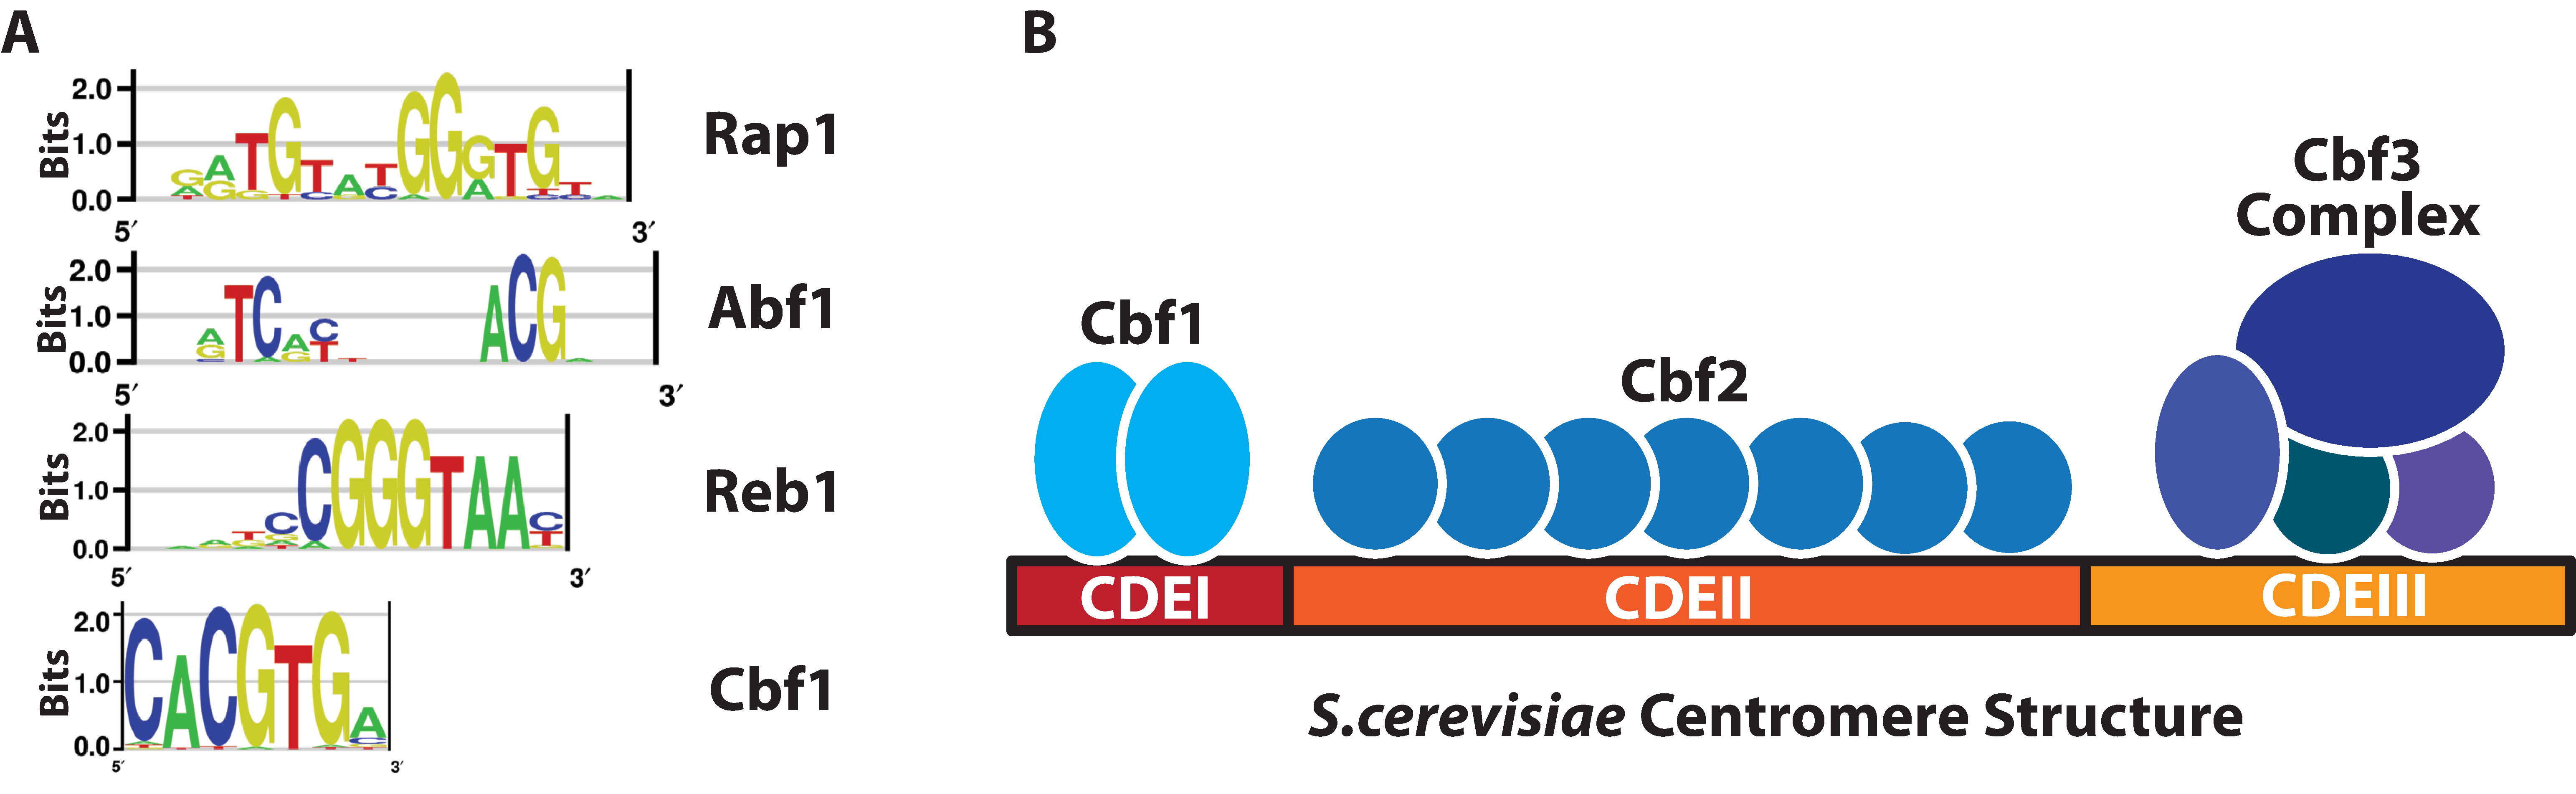
\includegraphics[width=\textwidth]{figures/introduction/grfCentromere}
\caption[GRFs binding sites and \cer{} centromere structure]{\textbf{A:} Sequence logos representing the main binding sites for the four GRFs Rap1, Abf1, Reb1, and Cbf1. \textbf{B:} structure of the centromere in \cer{} and its main interactors, A Cbf1 dimer is stably bound to CDEI.}
\label{fig:grfCentromere}

\end{figure}

\section{Rap1}

The essential transcription factor Rap1 is probably the best characterized GRF and it has a multitude of functions. 
Rap1 has a strong preference for the specific DNA element shown in figure \ref{fig:grfCentromere}A. This binding is mediated by two large DNA binding domains very similar to those of the human oncogene Myb \cite{rhee:2011:comprehensive}. 

Rap1 is the main transcriptional activator of ribosomal protein (RP) genes, controlling the expression of about 90\% of these species \cite{moehle:1991:association}. 
This regulation is enacted through multiple pathways.
First, Rap1 recruits a number of ancillary transcription factors: Fhl1, Ifh1, Sfp1, and Hmo1. Together they modify the structure of chromatin and stimulate transcription \cite{reja:2015:molecular}. 
Second, Rap1 is able to independently recruit TFIIA and TFIID to the promoter of RP genes, accelerating the rate of PIC formation at these loci \cite{papai:2010:tfiia}.


In addition to its activator capabilities, Rap1 works as an active silencer of transcription. 
During vegetative growth, the mating type loci of S.cerevisie are transcriptionally inactive. 
Their silencing is mediated by binding of Rap1, Orc1, and another GRF, Abf1. 
These proteins are able to recruit Sir1, Sir2, Sir3, and Sir4, which mediate the spread of heterocromatin over the HML and HMR loci, preventing transcription initiation \cite{kurtz:1991:rap1}. 
The transcriptional repressor activity of Rap1 has also been reported for RP genes under conditions of nutrient starvation, but in these conditions the silencing mechanism remains unclear \cite{reja:2015:molecular}. 


Lastly Rap1 has been implicated in the maintenance of telomeres \cite{lustig:1990:involvement}. 
In this context, Rap1 is part of a complex named Telosome together with Rif1 and Rif2. 
The telosome forms a protective cap around telomere sequences and is required for different aspects of telomere homeostasis such as telomere length regulation, inhibition of end resection, protection from fusion and inhibition of untimely activation of the DNA damage checkpoint \cite[for review see][]{wellinger:2012:everything}. 
Recent genome-wide studies identified Rap1 binding sites both at telomeres and RP genes, showing that these two classes of binding sites are distinct \cite{rhee:2011:comprehensive}. 
Somewhat consistent with this notion, another study showed how Rap1 possesses two binding modes. 
According to the authors, Rap1 can either bind a single site with high efficiency making use of both its Myb-like DNA binding domains, or it can bind more degenerate sequences with lower affinity using only one domain, but forming higher stoichiometry complexes \cite{feldmann:2014:dnabinding}. 
However, whether these two binding modes have functional consequences is unknown.

Rap1, together with other GRF such as Reb1 and Abf1, has been shown to have a role as as insulator (i.e. preventing the spread of heterochromatic silencing), and is thought to act in this capacity at the mating type loci \cite{fourel:2002:general}.


\section{Abf1}

Both Structurally and functionally close to Rap1, Abf1 is another essential factor implicated in numerous processes. 
Abf1 binds the split DNA site shown in figure \ref{fig:grfCentromere}A, which is known to regulate hundreds of promoters. 

While the vast majority of RP genes are regulated by Rap1, a cohort representing 10\% of the total is under the control of Abf1 \cite{dellaseta:1990:abf1}. 
A recent study investigated the mechanism of Abf1-dependent RP gene regulation, showing that Abf1 is found in association with Fhl1 and Ifh1, but has a lower occupancy on the promoter relative to Rap1 \cite{fermi:2016:multiple}. 
Abf1-dependent regulation of RP genes seems to possess distinct features from the canonical Rap1 regulation. 
Under nutrient starvation, Abf1 was observed to be more stably associated with the promoter and this resulted in a severe downregulation of gene expression. 
The authors speculated that stable association of Abf1 with DNA could mediate transcriptional silencing, while a more dynamic interaction could mediate activation \cite{fermi:2016:promoter}.

Akin to Rap1, Abf1 is known to act in silencing at the mating type loci, as well as an insulator in sub-telomeric regions \cite{mak:2009:dynamic}. 

Abf1 is present in a number of autonomous replicating sequences (hence the name ARS Binding Factor 1). 
These regions of the genome are essential to the process of DNA replication and act as its starting points.
The C-terminal region of Abf1 was found to enhance replicative activity independently of the transcription activation domain \cite{wiltshire:1997:abf1p}. 
In addition, replication factors have been shown to increase Abf1 DNA-binding activity \cite{feng:1998:saccharomyces}. 
Despite these data, however, Abf1’s mechanism of action at replication origins has never been fully elucidated.

Lastly, Abf1 is implicated in the activity of the global genome nucleotide excision repair mechanism (GG-NER). 
Abf1 was shown to form a stable complex with Rad7 and Rad16, two essential protein for GG-NER activity  \cite{reed:1999:yeast}. 
Additionally, impairing Abf1 DNA binding results in UV-sensitive yeast. 
The Rad7-Rad16-Abf1 complex is known to generate superhelical torsion in DNA \cite{yu:2004:yeast}, and Abf1 is thought to provide specificity to the complex through its DNA binding activity \cite{Yu:2009:abf1binding}.

\section{Reb1}

Reb1 was first identified as an rDNA enhancer binding protein, where it acts in stimulating transcription of ribosomal DNA \cite{planta:1995:global}. 
Reb1 tightly binds the consensus reported in figure \ref{fig:grfCentromere}A with a bipartite myb-like DNA binding domain.
Functionally, it acts to promote transcription of about 600 genes and it was implicated as an insulator in sub-telomeric regions. 
The homologue of Reb1 in S.pombe has been extensively studied as a DNA replication termination factor, as it is able to stall replication forks \cite{sa:2004:transcription}. The implication in this process in S.cerevisiae, however, is still unproven.


Reb1 was mistakenly believed to be the effector of RNAPI transcription termination \cite{lang:1995:transcription}. 
This notion, however, was dispelled when it was shown that Nsi1, a related protein that binds the same consensus on DNA, was the true molecular effector of RNAPI termination \cite{reiter:2012:reb1homologue}. 
Interestingly, Reb1 is now implicated in the termination of RNAPII through the same road-block mechanism with which it was thought to terminate RNAPI \cite{colin:2014:roadblock}.


\section{Cbf1}

Cbf1 is the only GRF thus far to not possess a myb-like DNA binding domain. Instead, it is a member of the helix-loop-helix family of DNA binding factors and specifically binds the consensus represented in figure \ref{fig:grfCentromere}A. 
Cbf1 is mostly known for its activity as a structural element in centromeres, but can stimulate transcription of a limited number of genes \cite{mellor:1990:cpf1}.


In S.cerevisiae, centromeres are short (120 nucleotides) DNA sequences coated with proteins that mediate assembly of the kinetochore and proper chromosome segregation during mitosis (Fig. \ref{fig:grfCentromere}B). 
Structurally, the centromere sequence is divided into three Centromere DNA Elements (CDE): CDEI, CDEII, and CDEIII. Cbf1 is the main binder of CDEI, a region of the centromere known to be important, but not essential for chromosome segregation \cite{niedenthal:1993:cpf1}. 

\begin{table}
\begin{tabular}[c]{cccp{4.9cm}}
\hline 
GRF & DNA-binding & \makecell{Chromatin\\Remodeling}  & Functions  \\
\hline 
Rap1 & bipartite Myb-like & multiple \cite{reja:2015:molecular} & RP genes activation, silencing of mating type loci, telomere maintenance \vspace{2mm} \\ 
Abf1 & Myb-like & RSC & RP genes activation, silencing of mating type loci, insulator, stimulator of DNA replication \vspace{2mm} \\
Reb1 & bipartite Myb-like & RSC & terminator of RNAPII, insulator \vspace{2mm} \\ 
Cbf1 & Helix-turn-helix & unknown & part of centromeres, transcriptional activator \\ 
\hline 

\end{tabular} 
\caption[characteristics of GRFs]{summary of GRF functions, binding sites and associated chromatin remodeling system.}
\label{tab:grfs}
\end{table}

Additionally, Cbf1 is known to form a complex with transcription factors Met4 and Met28. 
Through this complex, Cbf1 is able to target Met4 to genes involved in Sulphur metabolism \cite{oconnell:1995:role}. 
In addition to bringing Met4 to the promoter of MET genes, Cbf1 is also known to modify the structure of chromatin at MET and other gene loci through a still unknown mechanism.


\section{Chromatin Remodeling} 

A common feature of GRFs is the capability of altering the local chromatin structure in the vicinity of their binding sites. This mechanism is used to clear nucleosomes from promoters and thus stimulate transcription. 
As a general rule, GRFs are considered “obbligate synergizers”: they can weakly stimulate transcription on their own, but achieve a much greater effect when another weak activator binds the same promoter. 
The chromatin remodeling activity of GRFs is therefore thought to act as a force multiplier, allowing normally weakly binding transcriptional activators, who would not be able to bind a more chromatinized template, to be stably bound on DNA \cite{chasman:1990:yeast,bussemaker:2001:regulatory,pilpel:2001:identifying}.


Although all GRF described possess some level of chromatin remodeling activity, it is unclear whether this stems from use of a common system or multiple independent pathways. 
Studies implicated Reb1 and Abf1 in connection with the RSC complex \cite{hartley:2009:mechanisms}. 
To prove this point, the authors depleted Abf1 and Reb1, which resulted in a shrinkage of several NFRs.
Subsequent depletion of the catalytic subunit of the RSC complex, Sth1, showed that NFRs regulated by Reb1 and Abf1 are also regulated by RSC. 
In addition, the authors inserted a Reb1 site within an ORF and observed that an NFR could form depending on the presence of both Reb1 and of Sth1. 
These findings were confirmed by more recent investigations \cite{kubik:2015:nucleosome}, which found a large overlap between promoters regulated by Reb1 and Abf1 and promoters regulated by RSC. 
The same study, however, discovered a number of promoters where NFRs are generated in a Reb1- and Abf1-dependent manner, but independently of RSC, arguing for a more complex regulation mechanism. 



\subsection{Genome-Wide Effect on Chromatin Structure}

The stereotypical view of eukaryotic promoters is characterized by well-positioned +1 and -1 nucleosomes surrounding a 150+ stretch of poorly chromatinized DNA. 
This notion was challenged by a recent study that showed the existence of nucleosomal particles inside a large number of promoter NFRs \cite{kubik:2015:nucleosome}. 
These fragile nucleosomes (FN) are particularly sensitive to the amount of micrococcal nuclease (MNase) used to reveal nucleosome positioning in a genome-wide manner, and therefore went undetected until now. 
Analysis of the distribution of GRF binding sites inside promoters showed that fragile nucleosomes are significantly associated with GRF binding. 
Additionally, the GRF-associated chromatin remodeling complex RSC was implicated in the process, and insertion of GRF binding sites in previously unaffected promoters was shown to induce fragile nucleosome formation. 
For Reb1 and Abf1, the GRF binding site seems to coincide with the position of the fragile nucleosome, suggesting a kinetic competition between histones and GRFs. 
In the case of Rap1, however, the situation is less clear. The binding site was detected upstream of the fragile nucleosome, and often entailed the presence of two, not one, of these unstable particles. 
How such large NFR is generated and how fragile nucleosomes are maintained within it is still unknown. 


Another study recently investigated the effect of GRFs Rap1 and Abf1 on genome-wide chromatin assembly \cite{ganapathi:2011:extensive}.
While chromatin remodeling activity has been (expectedly) detected at directly regulated promoters, the two GRFs were shown to affect---albeit to a lesser extent---the chromatin structure of thousands of genes. 
Using thermosensitive mutants of Rap1 and Abf1 the authors analyzed genome-wide nucleosome occupancy.
Analysis of these datasets led to the conclusion that a modest but significant change in nucleosome disposition was occurring at a number of loci that were not described as regulated by either Rap1 or Abf1.
Upon further analysis, these promoters were found to be enriched in low affinity or degenerate Rap1 and Abf1 sites. 
This suggests that even low affinity binding of GRFs can contribute to the regulation of gene expression through a chromatin remodeling activity, and underscores the idea of GRFs as force multipliers---or enabler of transcription---on a much larger scale than previously thought. 



 

